\documentclass[border=3]{standalone}

\usepackage{tikz}
\usetikzlibrary{patterns,calc,angles,quotes,positioning,arrows}
\usetikzlibrary{math}


% ======================================= 
\begin{document}




% ======================================= V
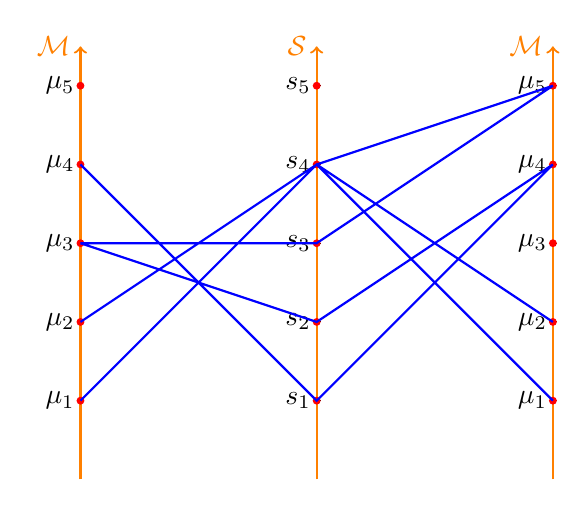
\begin{tikzpicture}

	\def\xMax{5}
	\def\yMax{5}
	\def\xMi{0}
	\def\xMj{6}
	\def\xS{3}
		
	% M i
	\draw [->,thick, orange]
		(\xMi, 0) -- (\xMi, {(\yMax+0.5)})
		node[anchor=east, xshift=-0 cm] {$\mathcal{M}$};
	\foreach \i in {1, ..., \yMax}{
		\draw 
			({(\xMi-0.05)}, \i) -- ({(\xMi+0.05)}, \i)
			node[anchor=east, xshift=-0 cm] {$\mu_{\i}$};
			\fill[red] (\xMi, \i) circle (0.05);
	}
	
	% S
	\draw [->,thick, orange]
		(\xS, 0) -- (\xS, {(\xMax+0.5)})
		node[anchor=east, xshift=-0 cm] {$\mathcal{S}$};
	\foreach \i in {1, ..., \xMax}{
		\draw 
			({(\xS-0.05)}, \i) -- ({(\xS+0.05)}, \i)
			node[anchor=east, xshift=-0 cm] {$s_{\i}$};
			\fill[red] (\xS, \i) circle (0.05);
	}
	
	% M j
	\draw [->,thick, orange]
		(\xMj, 0) -- (\xMj, {(\yMax+0.5)})
		node[anchor=east, xshift=-0 cm] {$\mathcal{M}$};
	\foreach \i in {1, ..., \yMax}{
		\draw 
			({(\xMj-0.05)}, \i) -- ({(\xMj+0.05)}, \i)
			node[anchor=east, xshift=-0 cm] {$\mu_{\i}$};
			\fill[red] (\xMj, \i) circle (0.05);
	}
	
	\draw [-,thick, blue]
		% Mi to S
		(\xMi, 4) -- (\xS, 1) -- (\xMj, 4)
		(\xMi, 3) -- (\xS, 2) -- (\xMj, 4)
		(\xMi, 3) -- (\xS, 3) -- (\xMj, 5)
		(\xMi, 2) -- (\xS, 4) -- (\xMj, 2)
		(\xMi, 1) -- (\xS, 4) -- (\xMj, 1)
		
%		(\xS, 1) -- (\xMj, 2)
		(\xS, 4) -- (\xMj, 5)
		(\xS, 4) -- (\xMj, 5)
		; % keep

\end{tikzpicture}
% ======================================= V


% ======================================= A
\end{document}